%!TEX root = ../cursustekst_fys6.tex

\chapter*{Inleiding}

Er zijn legio voorbeelden waarin trillingen en golven voorkomen. Als inleiding zullen we er hier een niet onaardige kort aanstippen. Aanschouw de volgende wonderbaarlijke vergelijkingen \ldots
\begin{eqnarray*}
\vec{\nabla}\cdot\vec{E}&=&\frac{\rho}{\epsilon_0}\\[3mm]
\vec{\nabla}\times\vec{E}&=&-\frac{\partial\vec{B}}{\partial t}\\[3mm]
\vec{\nabla}\cdot\vec{B}&=&0\\[3mm]
c^2\vec{\nabla}\times\vec{B}&=&\frac{\vec{j}}{\epsilon_0}+\frac{\partial\vec{E}}{\partial t}\\
\end{eqnarray*}
Je zal misschien zeggen dat ze je niets zeggen. Toch ken je alle vier de vergelijkingen op \'e\'en term na. Je bent waarschijnlijk gewoon niet vertrouwd met de symbolen en de compacte manier waarop ze zijn weergegeven.\footnote{Het symbool $\vec{\nabla}$ staat voor $\vec{\nabla}=\frac{\partial}{\partial x}\vec{e}_x+\frac{\partial}{\partial y}\vec{e}_y+\frac{\partial}{\partial z}\vec{e}_z$. Het is een operator. Ze wordt de nabla-operator genoemd. $\times$ staat voor het vectorproduct (de derde rechterhandregel ken je om de richting van de resulterende vector te bepalen) en $\cdot$ staat voor het scalair product.} De letters E en B zouden wel een \emph{lichtje} moeten doen branden; het gaat over elektrische en magnetische velden. De vergelijkingen vormen de fundamentele wetten van het elektromagnetisme en worden de wetten van Maxwell\footnote{James Clerk Maxwell (1831 - 1879)} genoemd.\footnote{De eerste wet is de wet van Coulomb, maar dan beschreven voor elektrische velden in plaats van met krachten. Het symbool $\rho$ staat hier niet voor massadichtheid maar voor ladingsdichtheid. De term $\vec{\nabla}\cdot\vec{E}$ wordt de divergentie van het elektrisch veld genoemd en beschrijft de mate waarin het veld in een punt in de ruimte wordt opgewekt. De wet geeft de relatie tussen een lading en het elektrisch veld dat ze genereert. $\epsilon_0$ is op $4\pi$ na gelijk aan de constante $k$ in de wet van coulomb: $k=\frac{1}{4\pi\epsilon_0}$.

De tweede wet is de elektromagnetische inductiewet. De term in het linkerlid wordt de rotor van het elektrisch veld genoemd. Ze meet in hoeverre het veld een vortex of draaibeweging vertoont. Het rechterlid geeft de verandering van het magnetisch veld aan. Er staat de afgeleide naar de tijd (de gekrulde delta $\partial$ kan je lezen als een $d$). Herinner je dat een bewegende magneet een stroom kan opwekken in een spoel. De stroom volgt een cirkel waarvan het vlak loodrecht op de bewegingsrichting van de magneet staat. 

De derde wet ken je ook. Ze zegt dat de divergentie van het magnetisch veld nul is. Met andere woorden kunnen er in een punt in de ruimte niet meer magnetische veldlijnen vertrekken dan dat er toekomen. Magnetische veldlijnen zijn gesloten of er zijn geen monopolen voor het magnetisme \ldots

Als we bij de vierde wet de tweede term in het rechterlid even wegnemen, en lezen dat $\vec{j}$ voor de stroomsterkte staat, dan staat hier de wet die je in het 5de onder de vorm $B=\frac{\mu_0}{2\pi}\frac{I}{d}$ hebt geleerd. Het is de wet van Biot-Savart. Ze geeft de relatie tussen de stroomsterkte en de sterkte van het magnetisch veld dat rond de draad wordt gegenereerd. Herinner je dat de veldlijnen concentrische cirkels waren en zie dat het linkerlid nu de rotor van dat magnetisch veld is. Het linkerlid meet dus de mate waarin het magnetisch veld rondgaat.} \footnote{\textit{Ceci n'est pas une voetnoot.}\footnotemark}\footnotetext{In de strikte betekenis van het woord wel, maar dan toch een van ondergeschikt belang.}

Dit is niet omdat hij ze heeft uitgevonden maar omdat hij -- naast die ene term die je niet kent er aan toegevoegd te hebben -- de verschillende bestaande wetten heeft samengevoegd. Zo eenvoudige, compacte vergelijkingen met symbolen die een lust zijn voor het oog, in een wiskundige taal die onze snaar van zuivere logica en abstractie doet trillen, omvatten en beschrijven een onwaarschijnlijke uitgebreide waaier van verschijnselen. Dat is fysica ten top!

In de vergelijkingen staat ook een $c$\ldots Juist ja, de $c$ van de lichtsnelheid. Op het eind van de 19de eeuw was er bij het opstellen van de vergelijkingen nog geen $c$ aanwezig. In de plaats van $c^2$ stond er $\frac{1}{\mu_0\epsilon_0}$ oftewel\footnote{Door $c$ in de vierde vergelijking te vervangen en de laatste term in het rechterlid weg te laten, herken je enigszins de jouw bekende formule $B=\frac{\mu_0}{2\pi}\frac{I}{d}$. De uitdrukking $2\pi d$ als omtrek van een cirkel zit vervat in $\vec{\nabla}\times\vec{B}$.}
\begin{equation}
	c=\frac{1}{\sqrt{\mu_0\epsilon_0}}.
\end{equation}
Maxwell kende echter de waarde van $c$ en zag de gelijkenis\ldots. Bovendien liet hij zien dat een golvend elektrisch en een golvend magnetisch veld dat zich met dezelfde waarde als de lichtsnelheid voortplantte, een oplossing was van de vergelijkingen\footnote{Deze voetnoot bekijk je beter wanneer we het hoofdstuk over golven achter de rug hebben. En zelfs dan is hij niet zomaar te verstaan\ldots Maar we lopen hier toch even voor op de feiten. In het luchtledige reduceert de eerste vergelijking tot $\vec{\nabla}\cdot\vec{E}=0$ en de laatste tot $c^2\vec{\nabla}\times\vec{B}=\frac{\partial\vec{E}}{\partial t}$. Er zijn dan immers geen ladingen en geen stromen. Net iets geavanceerder rekenen met $\vec{\nabla}$ levert, als we slechts \'e\'en dimensie beschouwen, de vergelijking $\frac{\partial^2E}{\partial t^2}=c^2\frac{\partial^2E}{\partial x^2}$ op. Dit is een golfvergelijking met $E=E_0\sin(kx -\omega t)$ als mogelijke oplossing als $c=\lambda f$. Dit kan je nagaan door in te vullen. De oplossing is dus een golf die zich met de lichtsnelheid voortbeweegt!}. Dat wilde zeggen dat hij dus een tot dan toe onverklaarbaar verschijnsel als het licht kon verklaren met een elektromagnetische golf. En dit als \emph{gevolg} van de opgestelde wetten. Om het in zijn eigen woorden te zeggen:
\begin{quotation}
\emph{This velocity is so nearly that of light, that it seems we have strong reasons to conclude that light itself [\ldots] is an electromagnetic disturbance in the form of waves propagated through the electromagnetic field according to electromagnetic laws.}
\end{quotation}
Het ongelofelijk knappe hiervan is dat die wetten hun oorsprong vinden in verschijnselen die daar op het eerste zicht niets mee te maken hebben: het aantrekken en afstoten van ladingen, magneten en stromen. Deze verschijnselen zijn in de eeuwen daarvoor onderzocht en door verschillende grote fysici in wetmatigheden gegoten om vervolgens, als bijkomende consequenties, ook licht, radiogolven, gsm-straling en alle andere golven binnen het elektromagnetische spectrum te kunnen beschrijven. Dat is binnen de fysica alweer een staaltje van unificatie!
%\newline
%\newline
%Zo zien we dat golven fundamentele natuurverschijnselen zijn. De moeite om te bestuderen dus\ldots 
%\newline
%\newline
%- E induceert B en omgekeerd
%- nabla uitschrijven

\newpage

\chapter{Harmonische trillingen}

Om golven te kunnen beschrijven, behandelen we eerst trillingen. Dat is een iets eenvoudiger verschijnsel. Trillingen zijn heen en weer gaande bewegingen op een lijn. Zo trilt bijvoorbeeld een gitaarsnaar wanneer je hem aanslaat, trilt het rietje in een hobo bij het blazen of trillen elektronen in de antenne van je gsm.


% \section{Enkele voorbeelden}
% 
% - geluid
% - licht
% - ht is sinus

\section{De harmonische oscillator}

Als eerste voorbeeld behandelen we een eenvoudig mechanisch systeem: een massa die aan een veer is bevestigd. We noemen dit een massa-veersysteem. En zoals we al zo vaak hebben gedaan, beschouwen we een model waar geen wrijving aanwezig is. Laten we bovendien de veer een horizontale ori\"entatie geven zodat we ook de zwaartekracht buiten beschouwing kunnen laten.
\begin{figure}[h]
\centering
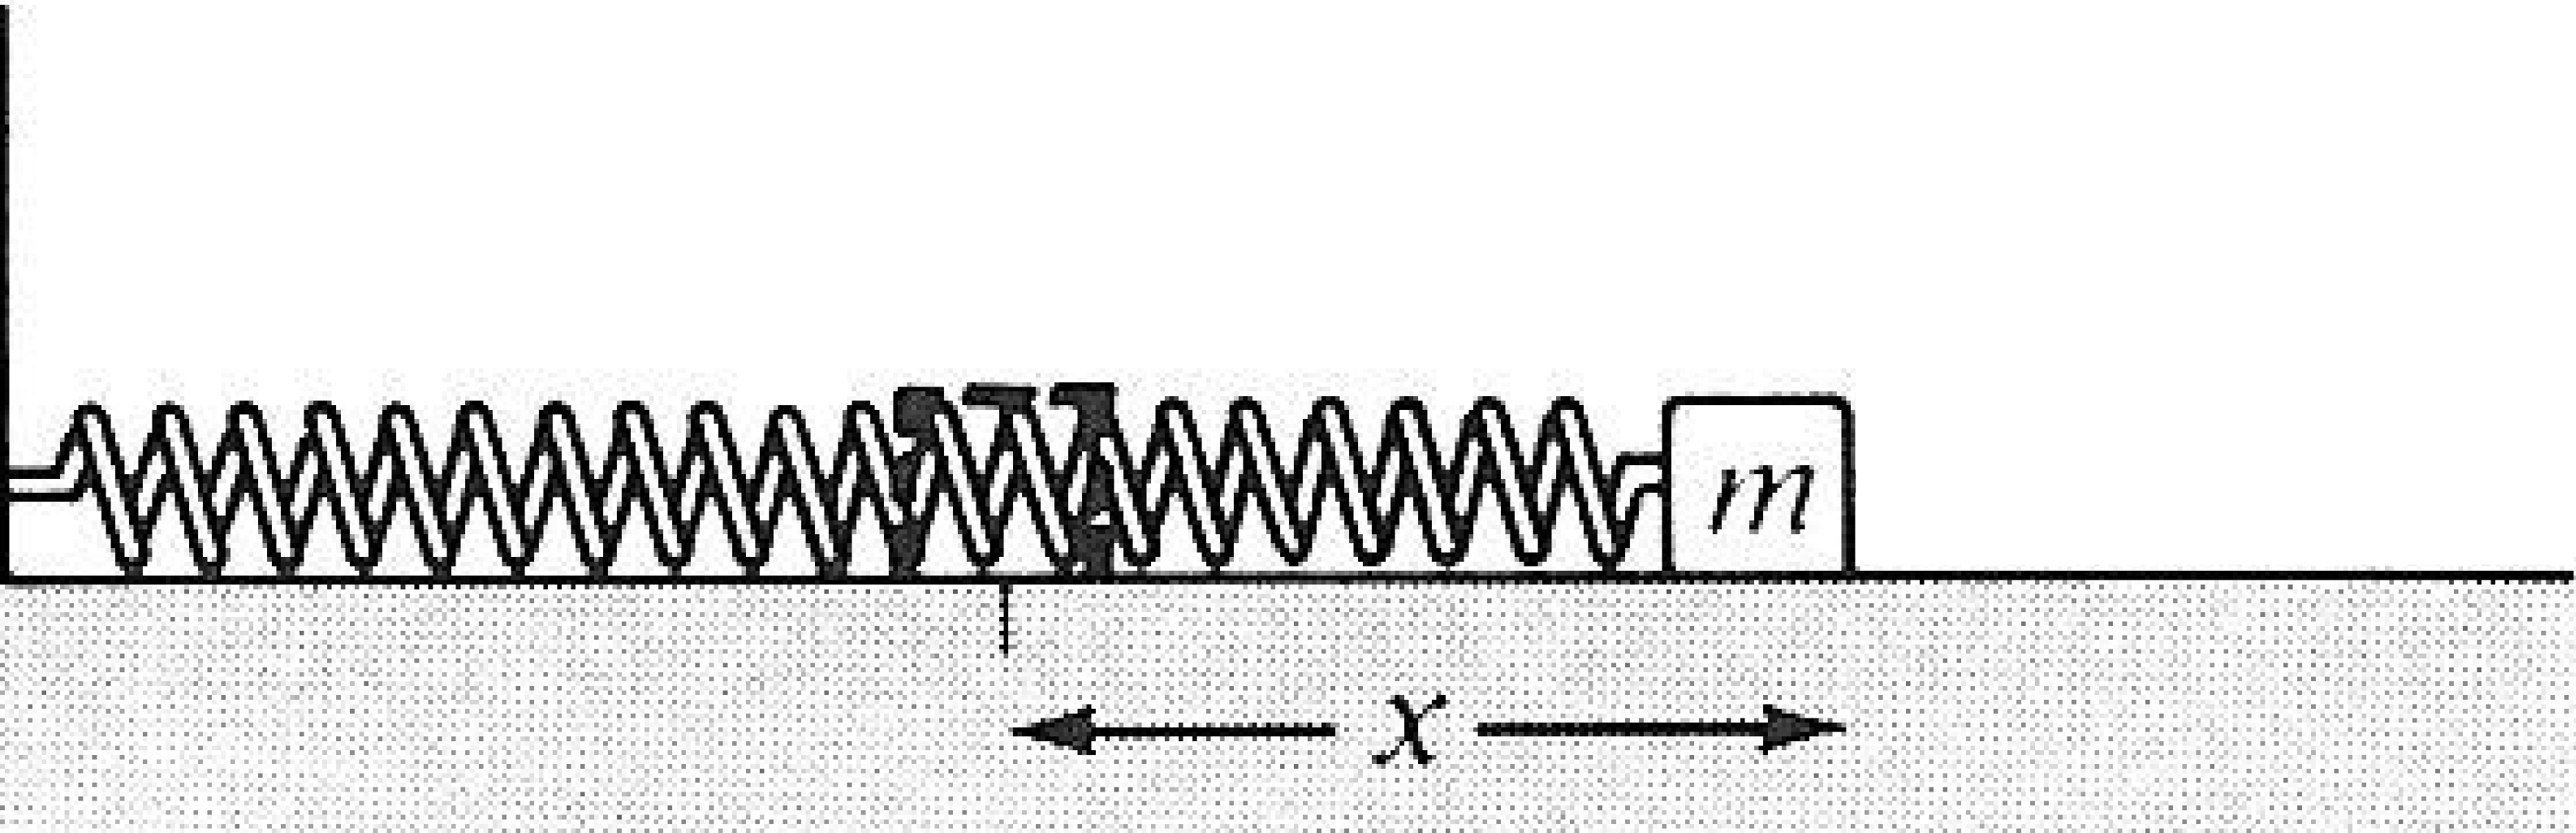
\includegraphics[width=0.8\textwidth]{kogeltegenveer2}
\end{figure}
Wanneer we de massa uit de positie halen waar de veer zijn rustlengte heeft en hem vervolgens loslaten, voert de massa een trilling uit. We constateren dat hij heen en weer beweegt waarbij hij steeds door de evenwichtspositie gaat. Deze beweging willen we natuurlijk uit onze natuurwetten tevoorschijn zien komen. Meer bepaald moet de tweede wet van Newton -- ons beginsel der beginselen in de klassieke mechanica -- de beweging opleveren. De trilling is een mechanisch verschijnsel en moet dus te verklaren zijn met behulp van die natuurwetten. 

Om de beweging te kunnen vinden, moeten we het systeem vrij maken -- alle krachten erop tekenen. We hebben dus de resulterende kracht nodig. Omdat het lichaam op een ondergrond rust en geen verticale versnelling heeft, heffen de normaalkracht en de zwaartekracht elkaar op. De resulterende kracht is bijgevolg de veerkracht. We gebruiken de wet van Hooke en gieten de component van de kracht volgens de bewegingsrichting in de vorm zoals we ze al kennen:\footnote{Deze beschrijving van de veerkracht is natuurlijk een benadering. Ze is maar geldig voor zolang de veer een niet te grote uitwijking kent. Het minteken zorgt voor een terugroepkracht; wanneer de co\"ordinaat $x$ positief is, is de component van de kracht negatief en wanneer de co\"ordinaat negatief is, is de component positief.}
\begin{eqnarray*}
F(x)=-kx
\end{eqnarray*}
Nu dat we ons model voor het massa-veersysteem hebben, kunnen we opzoek naar de beweging die de massa uitvoert. Hoe ziet de trilling er precies uit? De tweede wet van Newton dus \ldots
\begin{eqnarray}
F&=&ma\nonumber\\
&\Downarrow&\nonumber\\
-kx&=&m\frac{d^2x}{dt^2}\nonumber\\
&\Updownarrow&\nonumber\\
\frac{d^2x}{dt^2}+\frac{k}{m}x&=&0\label{diffvgl_ht}
\end{eqnarray}
\ldots\,en toen kwamen we uit bij een \ldots\,\emph{differentiaalvergelijking}. Om meer precies te zijn: een tweede-orde lineaire differentiaalvergelijking met constante co\"effici\"enten. Dat klinkt redelijk ingewikkeld. In feite is het ook niet zo simpel. We zijn opzoek naar de beweging, wat betekent dat we de positie $x$ in functie van de tijd willen vinden -- de functie $x(t)$ dus. De vergelijking die we gevonden hebben is niet zozeer een algebra\"ische vergelijking in een onbekende variabele $x$ (zoals bijvoorbeeld een tweedegraadsvergelijking) dan wel \emph{een vergelijking voor een functie}!\footnote{Wanneer we de impliciete afhankelijkheid van de tijd expliciet aangeven,ziet de vergelijking er als volgt uit
\begin{eqnarray*}
\frac{d^2x(t)}{dt^2}+\frac{k}{m}x(t)=0
\end{eqnarray*}} We zoeken dus een functie die aan de vergelijking voldoet. Een functie die voldoet is dan een oplossing van de vergelijking en dus een mogelijke beweging die de massa kan volgen. We spreken hier in eerste instantie over \emph{een} oplossing omdat er a priori\footnote{Vooraf beschouwd. Zonder het gezien, ervaren of onderzocht te hebben.} verschillende oplossingen kunnen zijn.

Het oplossen van differentiaalvergelijkingen is bijna een stiel op zich. Want dergelijke vergelijkingen zijn er in alle maten, geuren, kleuren en vooral moeilijkheidsgraden. En aangezien we die cursus willen overlaten aan degene die zich bij verdere studies hierin wil verdiepen, hebben wij op dit moment geen directe manier om tot de oplossingen te komen. Dat betekent dat we hier iets creatiever zullen moeten zijn en de methode van het ge\"inspireerd gokken zullen moeten toepassen \ldots In de modus van minder hoge ambities, kunnen we in eerste instantie een functie uit onze hoed toveren en nagaan of ze een oplossing is. Dat is natuurlijk onbegonnen werk wanneer we \'alle functies nagaan\footnote{Zoals het ook voor een schaakcomputer onbegonnen werk zou zijn, moest hij alle mogelijke zetten evalueren om de beste er uit te kunnen pikken.} maar haalbaar wanneer we ons fysisch inzicht erbij halen\footnote{Zoals ook een schaker alleen maar die paar zetten bestudeert waarvan hij ziet dat ze de moeite waard zijn.}. Zo moet de functie de beweging beschrijven en zullen de vergelijkingen voor een EVRB naar alle waarschijnlijkheid niet voldoen. De massa gaat heen en weer zodat we met een functie te maken moeten hebben die dat ook doet. Waarom zou dus een \emph{sinusfunctie} niet voldoen \ldots?!
\begin{figure}[h]
\centering
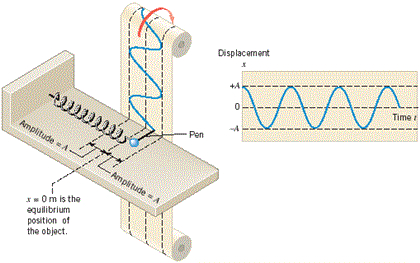
\includegraphics[width=.6\textwidth]{ht_papierrol}
\end{figure}

Om te proberen nemen we een eenvoudige sinusfunctie $x(t)=\sin\omega t$. Bij het invullen in de vergelijking (\ref{diffvgl_ht}) moeten we voor de eerste term in het linkerlid de tweede afgeleide berekenen; $x''(t)=-\omega^2\sin\omega t$. De tweede term geeft bij het invullen $\frac{k}{m}\sin\omega t$. Wil nu de voorgestelde functie een oplossing zijn, dan moet hetgeen we verkregen hebben, gelijk zijn aan het rechterlid -- namelijk nul.
\begin{eqnarray*}
 -\omega^2\sin\omega t+\frac{k}{m}\sin\omega t=0\Leftrightarrow\left(-\omega^2+\frac{k}{m}\right)\sin\omega t=0\Leftrightarrow\omega^2=\frac{k}{m}
\end{eqnarray*}
In de laatste overgang hebben we gebruik gemaakt van het feit dat de sinus welliswaar nul kan worden maar dit nooit voor \'alle tijdstippen het geval is. De vergelijking moet altijd opgaan -- niet enkel voor een paar momenten in de tijd. Wanneer we dus $\omega=\sqrt{k/m}$ nemen, is de voorgestelde functie een oplossing van de differentiaalvergelijking. We hebben zowaar een mogelijke beweging gevonden die de massa kan uitvoeren!

Natuurlijk hebben we nu slechts \emph{een} oplossing. Misschien zijn er nog. Want, waarom zou een cosinusfunctie niet voldoen? Een cosinusfunctie kunnen we beschrijven als een verschoven sinusfunctie zodat een sinusfunctie in algemene vorm $x(t)=a\sin(b(t-c))+d$ het proberen waard is. We kiezen voor het gemak $d$ gelijk aan nul\footnote{Dit komt overeen met het plaatsen van de oorsprong in de evenwichtspositie van de massa.} en geven in deze context de andere parameters andere symbolen: $a$ vervangen we door $A$, $b$ door $\omega$ en $-bc$ door $\varphi$. Die parameters hebben nl. een iets meer fysische betekenis -- waarover later meer. Ga nu na\footnote{Doe dit effectief. En nee, al liggend in je bed en kijkend naar dit blad voldoet niet aan de imperatief. Iets nagaan in deze exacte wereld van wiskunde en natuurkunde doet men met pen en papier / bord en krijt. Eventueel bijgestaan door een computer.} dat de functie 
\begin{eqnarray*}
x(t)=A\sin(\omega t+\varphi)\quad\mathrm{met}\quad\omega=\sqrt{\frac{k}{m}}
\end{eqnarray*}
een oplossing is van de differentiaalvergelijking. In feite is dit de algemene oplossing van de differentiaalvergelijking. Hier hebben we de existentie aangetoond; het feit dat er een oplossing bestaat. De uniciteit ervan -- het feit dat er geen andere functie bestaat -- is nog een ander paar mouwen.

Samengevat vinden we dat voor een lineaire terugroepkracht $F=-kx$ de beweging een harmonische trilling is. Ook het omgekeerde is waar: voert een lichaam een harmonische trilling uit, dan is de kracht lineair en steeds naar de oorsprong gericht.
\begin{eqnarray}
\frac{d^2x}{dt^2}+\frac{k}{m}x&=&0\nonumber\\
&\Updownarrow&\nonumber\\
x(t)=A\sin(\omega t+\varphi)\quad&\mathrm{met}&\quad\omega=\sqrt{\frac{k}{m}}\label{opl_diffvgl_ht}
\end{eqnarray}
We hebben nu de wiskundige oplossing van de differentiaalvergelijking gevonden. De massa trilt sinuso\"idaal in de tijd. Vandaar dat we over een harmonische trilling spreken.

De verschillende parameters die in de oplossing (\ref{opl_diffvgl_ht}) voorkomen, willen we fysisch kunnen interpreteren. We willen hun betekenis kennen. Het gemakkelijkste is misschien terug te grijpen naar de algemene sinusfunctie. Daar stond de parameter $a$ voor de amplitude. Dat is dus hier voor $A$ niet anders; $A$ stelt de amplitude van de trilling voor. Voor de parameter $b$ hebben we de gelijkheid $b=\frac{2\pi}{p}$ waarin $p$ de periode van de functie is. Omdat onze onafhankelijke variabele de tijd is, is de fysische interpretatie van $p$ de tijd van \'e\'en cyclus -- waarvoor we het symbool $T$ gebruiken. 
\begin{figure}[h]
\centering
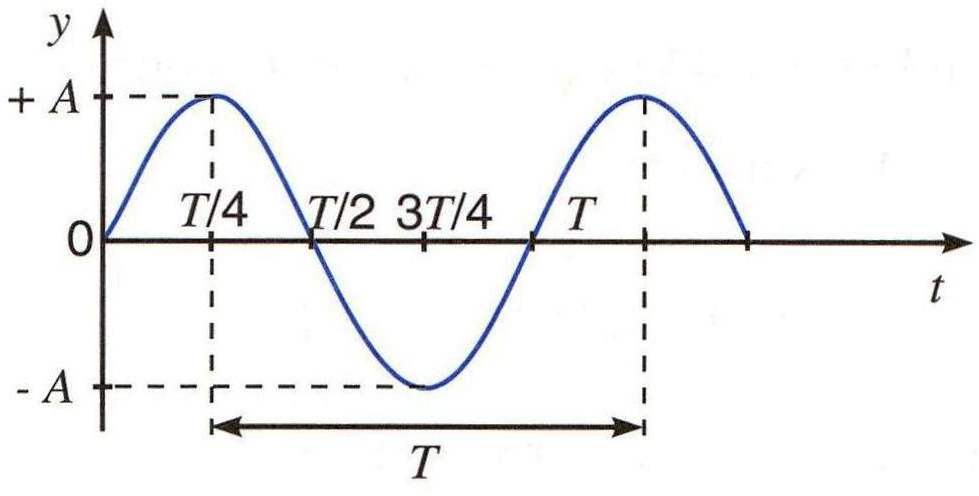
\includegraphics[width=.7\textwidth]{ht_tijd}
\end{figure}
Voor de parameter $\omega$, die we de pulsatie noemen, geldt dus
\begin{eqnarray*}
\omega=\frac{2\pi}{T}
\end{eqnarray*}
De pulsatie bepaalt dus de frequentie waarmee de massa trilt. Aangezien voor het massa-veersysteem geldt dat $\omega=\sqrt{k/m}$, kunnen we een uitdrukking voor periode en de frequentie vinden:
\begin{eqnarray*}
T=2\pi\sqrt{\frac{m}{k}},\quad f=\frac{1}{2\pi}\sqrt{\frac{k}{m}}
\end{eqnarray*}
De frequentie wordt bepaald door de sterkte van de veer en de grootte van de massa. Een grotere massa levert een kleinere frequentie op (de traagheid is groter) en een sterkere veer zorgt voor een grotere frequentie (de massa krijgt een grotere versnelling). De amplitude speelt blijkbaar geen rol.

De parameter $\varphi$ is iets lastiger om inzichtelijk te kunnen duiden. Net zoals de amplitude wordt ze bepaald door de \emph{beginvoorwaarden}. Zo is de amplitude afhankelijk van bijvoorbeeld de afstand uit de evenwichtspositie waarop we de massa vanuit rust loslaten of van de snelheid die we ze bij initiatie van de beweging meegeven. De parameter $\varphi$ wordt bepaald door de positie van de massa op het tijdstip $t=0$. Immers is $x_0=x(t=0)=A\sin(\varphi)$. Het argument van de sinus\footnote{Het argument van de sinus is hetgeen waarvan de sinus wordt genomen/hetgeen dat tussen haakjes staat.} $\omega t+\varphi$ noemen we ook wel de \emph{fase} van de trilling zodat $\varphi$ de \emph{beginfase} wordt genoemd. De fase drukken we natuurlijk uit in radialen. De fase bepaalt waar we ons in de cyclus bevinden. 
%\begin{figure}[h]
%\centering
%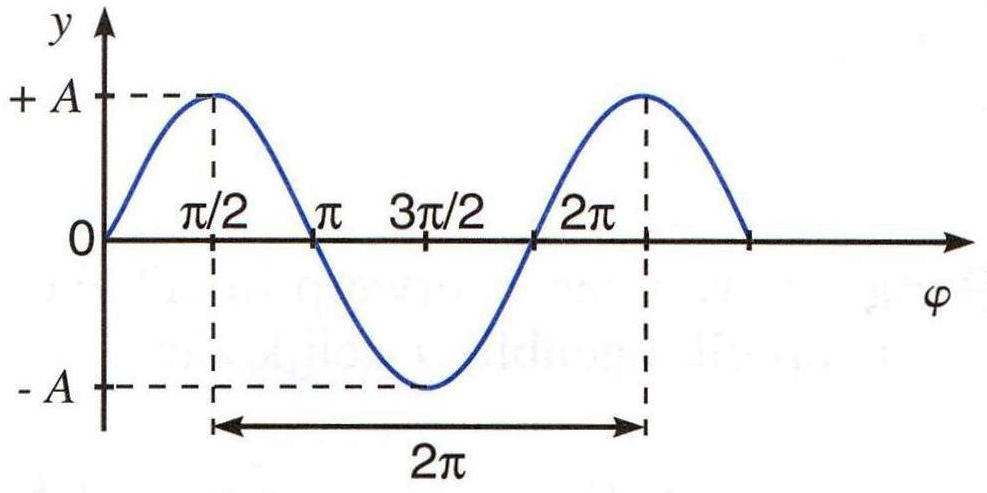
\includegraphics[width=.7\textwidth]{ht_fase}
%\end{figure}
%\newline
De beginfase bepaalt dan ook de beginpositie. Zo is bijvoorbeeld de functie maximaal wanneer het argument $\pi/2$ is, wat betekent dat de massa op haar maximale uitwijking is. Is dus de beginfase gelijk aan $\pi/2$, dan begint de trilling vanuit haar maximale uitwijking. Een beginfase van $3\pi/2$ komt overeen met een minimale waarde bij het begin. In figuur \ref{beginposbeginfase} zie je verschillende mogelijkheden voor de beginfase, hier weergegeven als $\varphi_0$.

Nu dat we de positie in functie van de tijd kennen, vinden we door af te leiden de snelheid en de versnelling van de massa. 
\begin{eqnarray*}
x&=&A\sin(\omega t+\varphi)\\[3mm]
v=\frac{dx}{dt}&=&\omega A\cos(\omega t+\varphi)\\[3mm]
a=\frac{d^2x}{dt^2}&=&-\omega^2A\sin(\omega t+\varphi)=-\omega^2x
\end{eqnarray*}
Merk op dat de versnelling op een constante ($\omega^2$) na tegengesteld is aan de positie. Dat is niet verwonderlijk aangezien we te maken hebben met de wet van Hooke en volgens de tweede wet van Newton de versnelling recht evenredig is met de kracht. 

\newpage

\begin{figure}
	\centering
	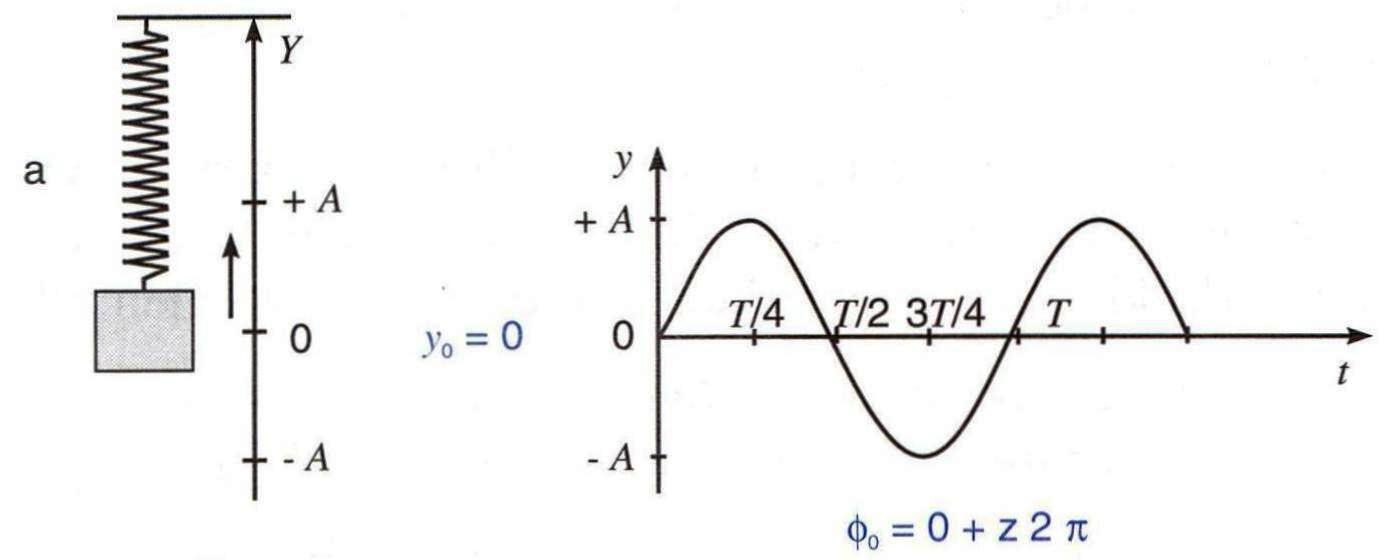
\includegraphics[width=.9\textwidth]{trillendeveer_a}
	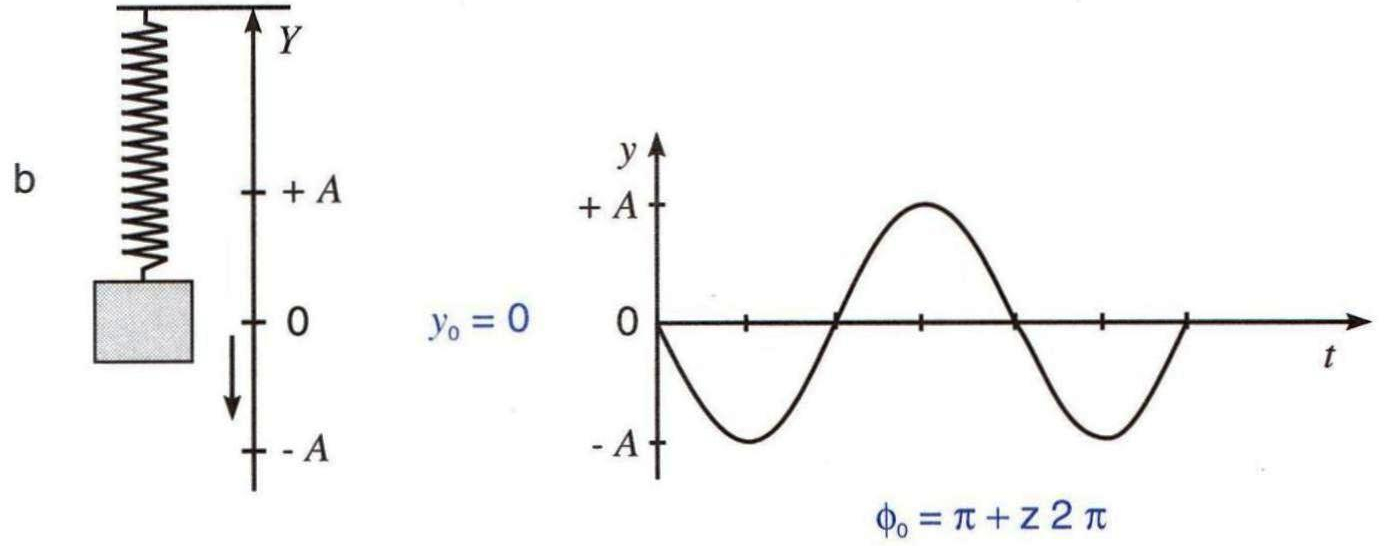
\includegraphics[width=.9\textwidth]{trillendeveer_b}
	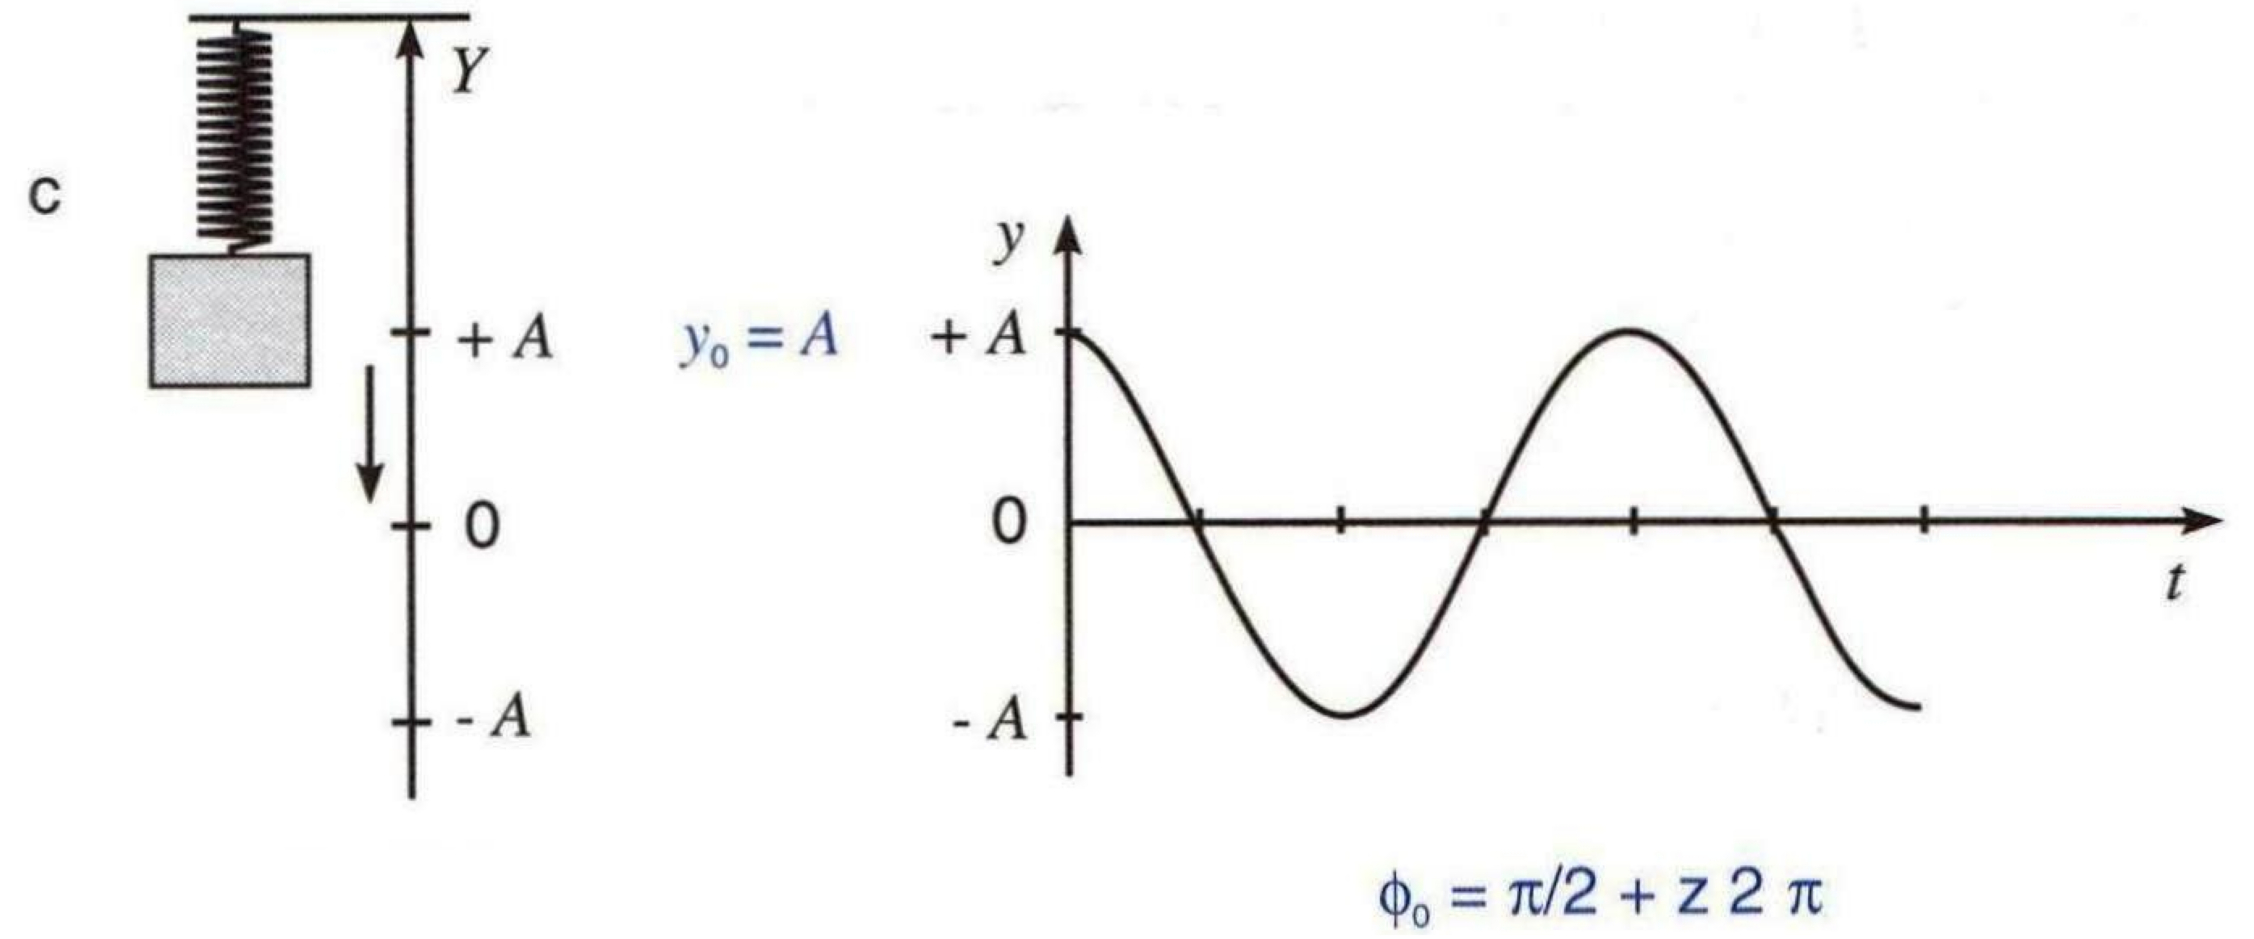
\includegraphics[width=.9\textwidth]{trillendeveer_c}
	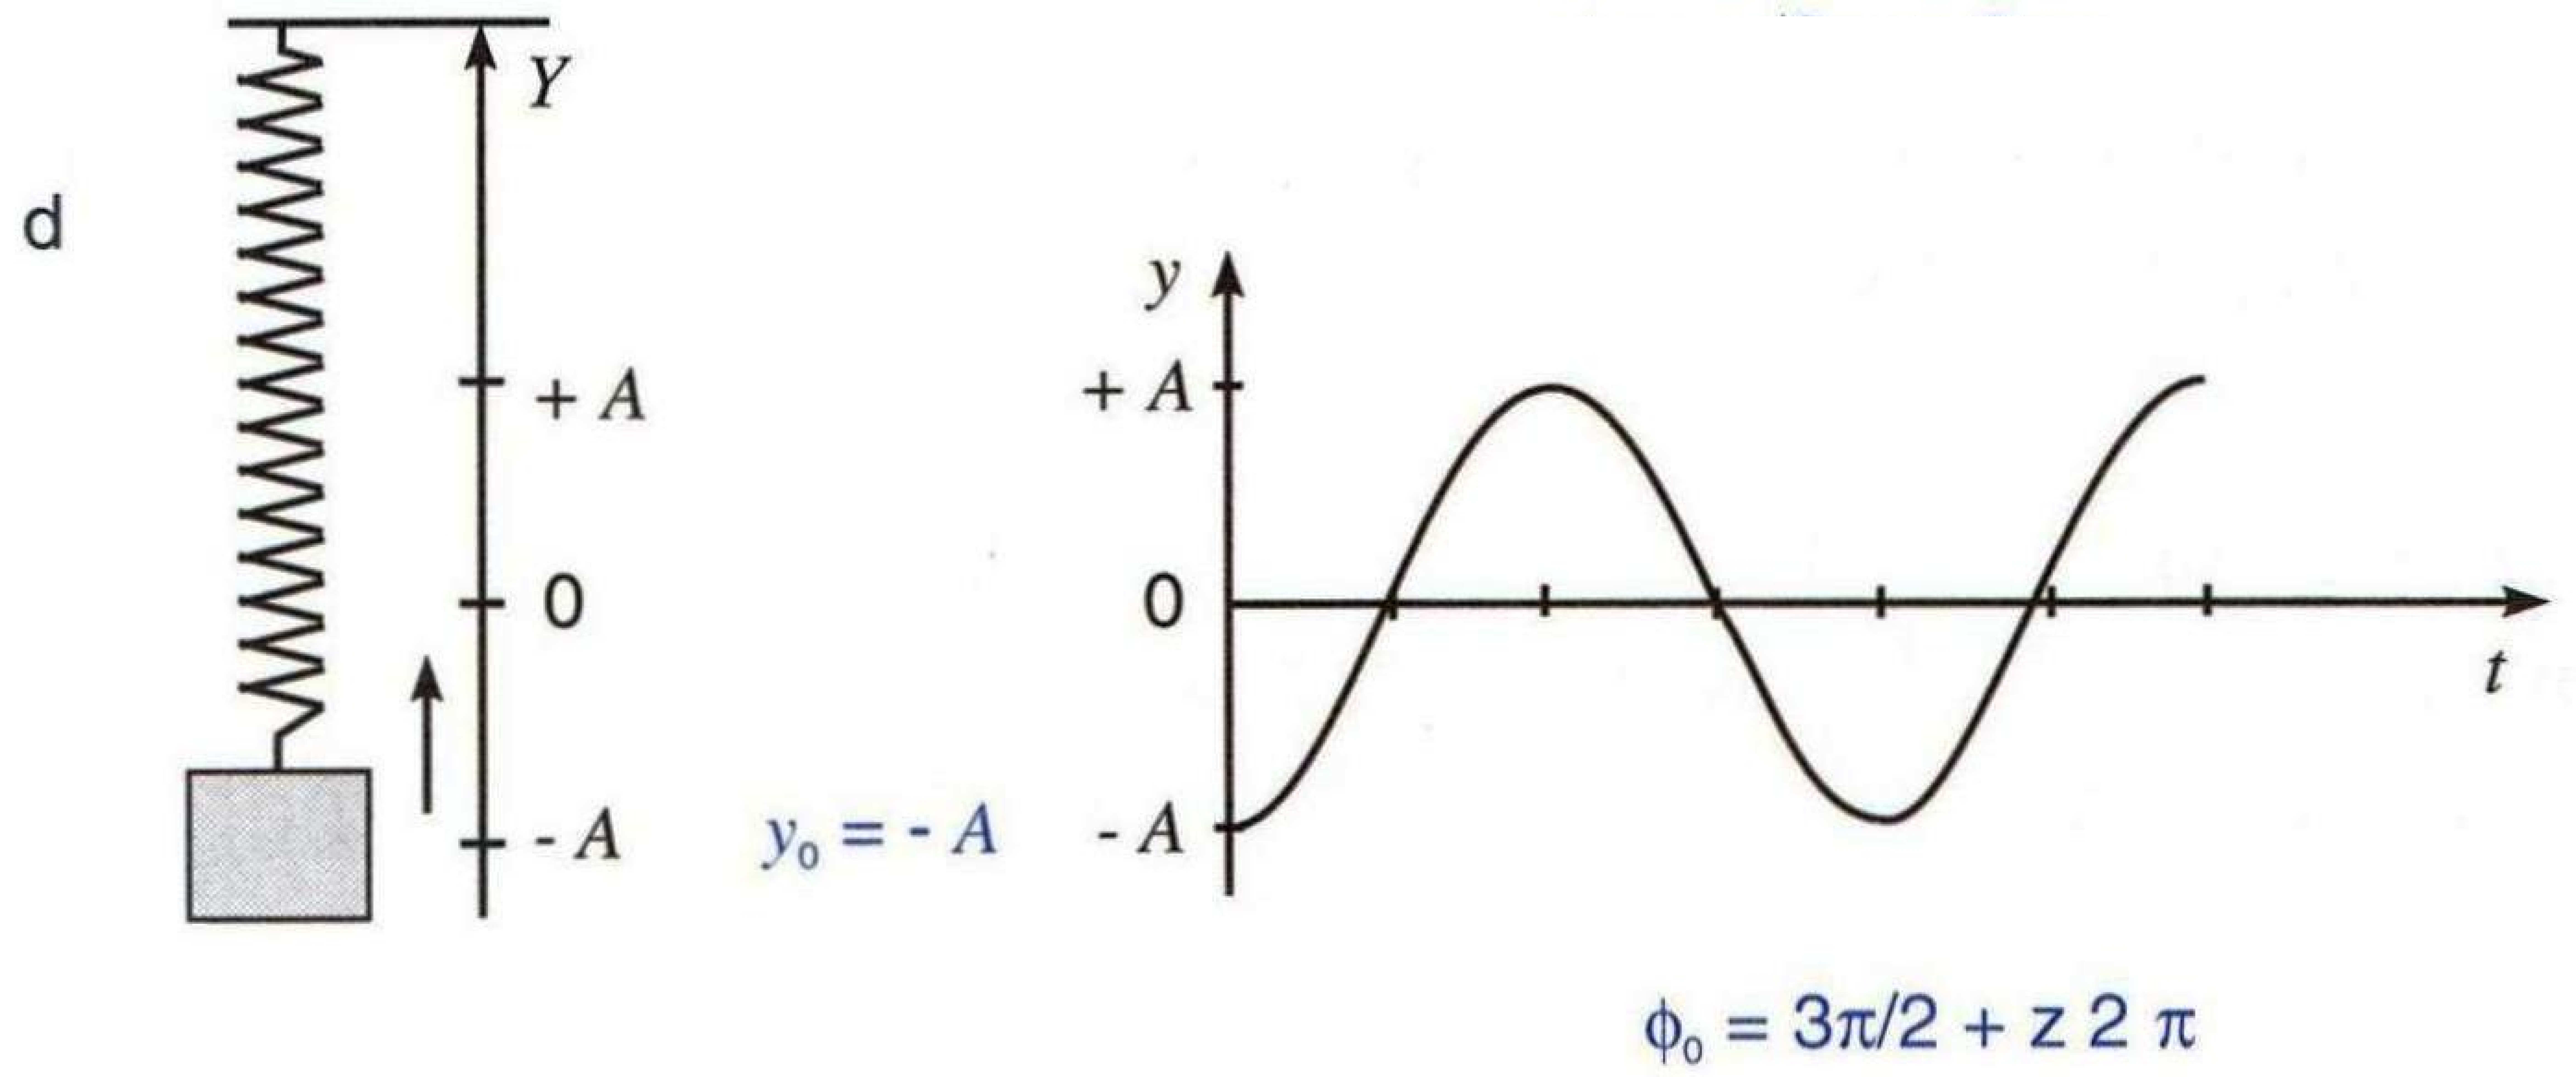
\includegraphics[width=.9\textwidth]{trillendeveer_d}
	\caption{Relatie tussen beginpositie en beginfase}
	\label{beginposbeginfase}
\end{figure}

\clearpage
\newpage

Naast in detail de beweging te hebben bestudeerd, kunnen we ook naar het energieverloop kijken. Hiertoe vullen we gewoonweg de positie en de snelheid in de formules voor energie in.
\begin{eqnarray*}
E_k&=&\frac{mv^2}{2}=\frac{1}{2}m\omega^2A^2\cos^2(\omega t+\varphi)\\
E_p&=&\frac{1}{2}kx^2=\frac{1}{2}kA^2\sin^2(\omega t+\varphi)=\frac{1}{2}m\omega^2A^2\sin^2(\omega t+\varphi)
\end{eqnarray*}
Deze hangen duidelijk af van de tijd. Wanneer we naar de totale energie kijken, vinden we -- zoals we volgens de wet van behoud van energie mogen verwachten -- dat deze constant is.
\begin{eqnarray*}
E=E_k+E_p=\frac{1}{2}m\omega^2A^2\left(\sin^2(\omega t+\varphi)+\cos^2(\omega t+\varphi)\right)=\frac{1}{2}m\omega^2A^2
\end{eqnarray*}
\begin{figure}[h]
\centering
%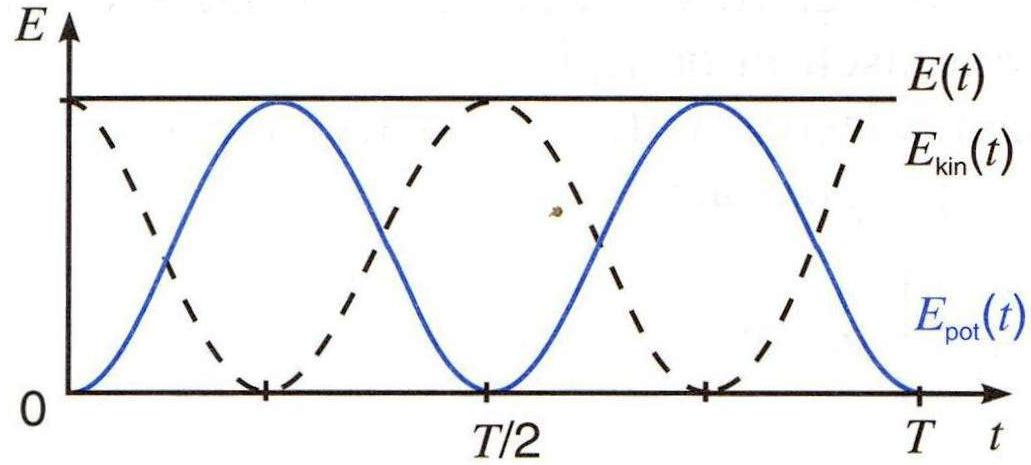
\includegraphics[width=.7\textwidth]{EpEkE}
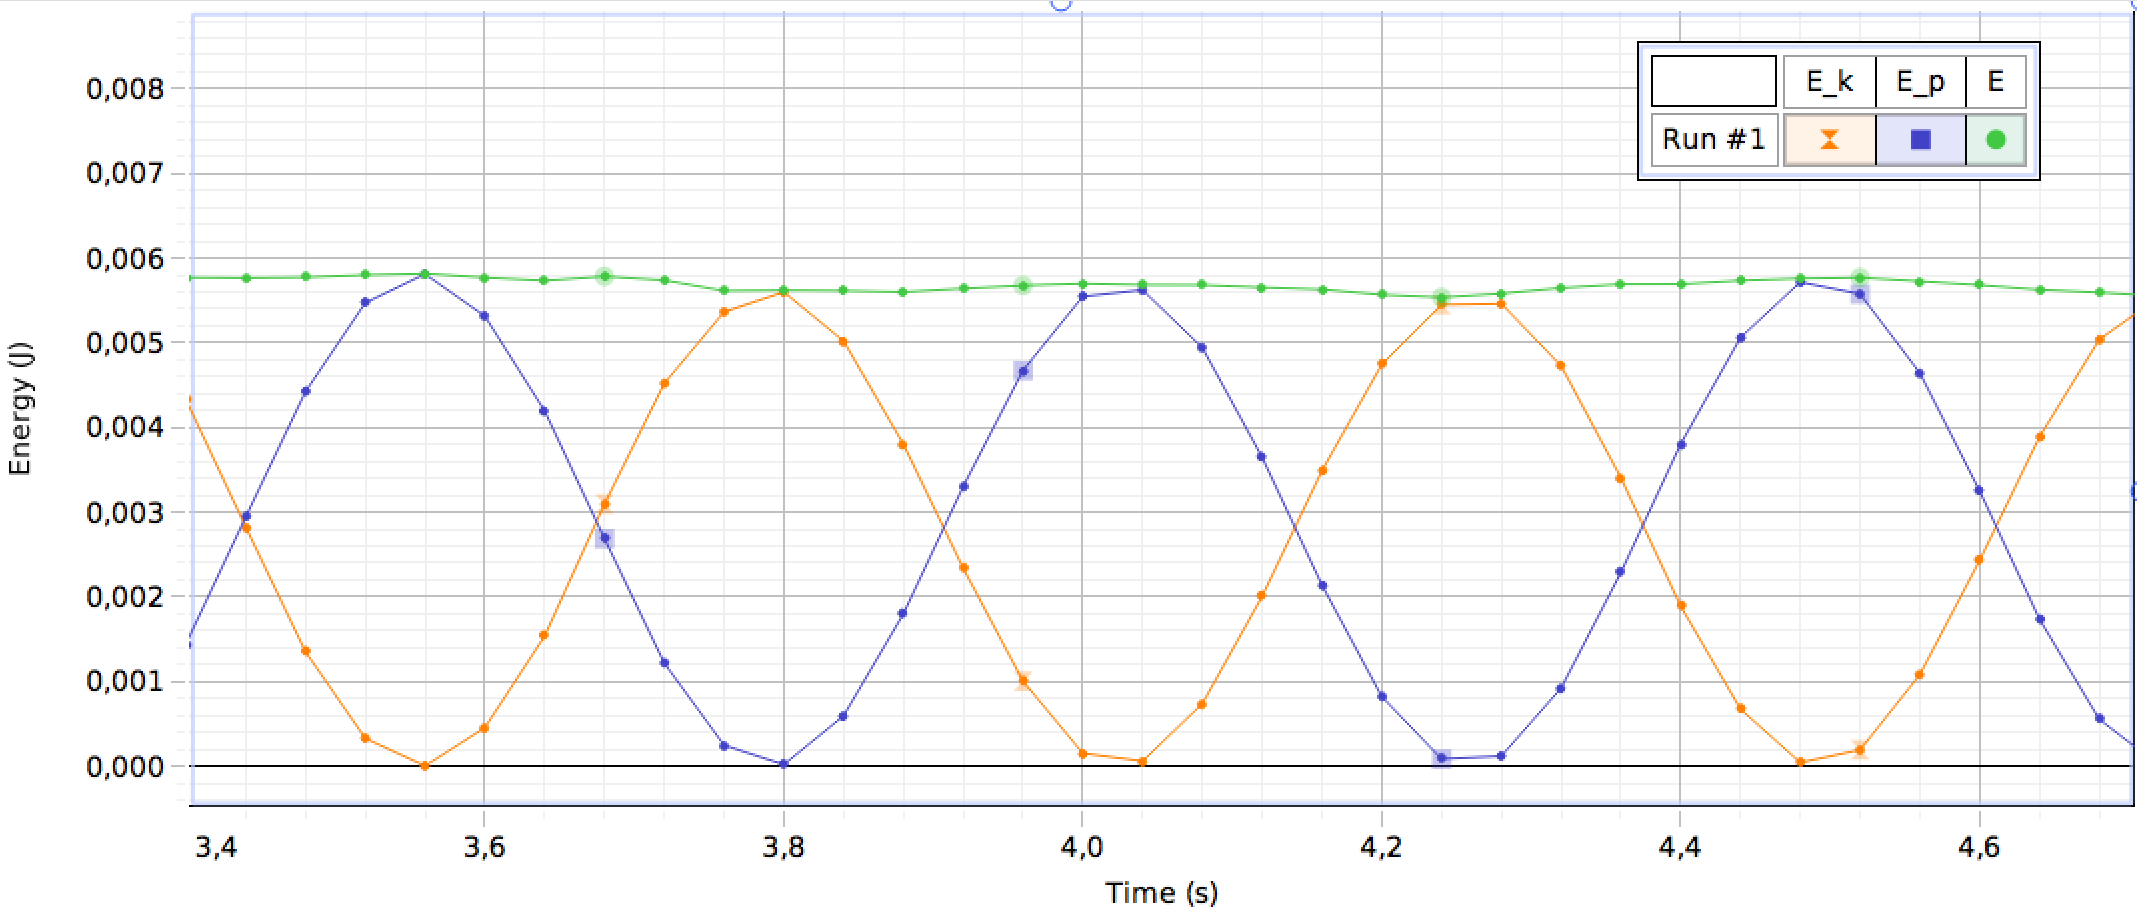
\includegraphics[width=.9\textwidth]{ht_behoud_energie}
\end{figure}
Merk op dat de energie van een trilling recht evenredig is met het kwadraat van de amplitude. Een golf in de zee die dus twee keer zo hoog is, draagt vier keer zoveel energie met zich mee. In de figuur zie je mooi hoe de kinetische en de potenti\"ele energie in elkaar worden omgezet; het verlies van de ene is de winst van de andere. Let op het verschil tussen de periode van de energievormen en de periode van de eigenlijke trilling \ldots

%\newpage

\section{Relatie met een cirkelbeweging}

Wanneer we op een grammofoonplaat en klein object leggen en met een lamp de schaduw op de muur bekijken terwijl de plaat draait, dan zien we evenzeer een op- en neergaande beweging. 
\begin{figure}[h]
%\centering
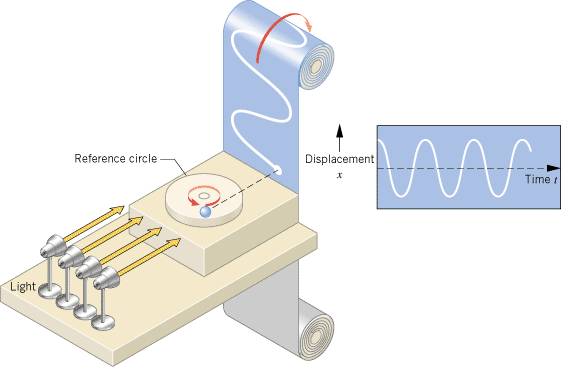
\includegraphics[width=.6\textwidth]{ht_schaduw}
\hspace{5mm}
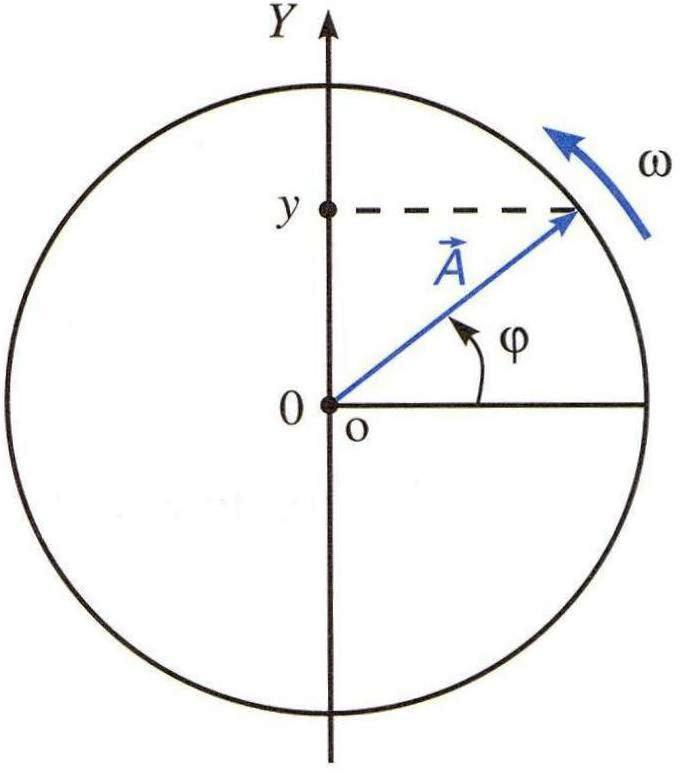
\includegraphics[width=.35\textwidth]{fasor}
\end{figure}
Het gaat hier echter ook om een harmonische trilling. Bekijken we immers de $y$-co\"ordinaat van een punt op een cirkel dat met een constante hoeksnelheid beweegt, dan is dit een sinusfunctie. Als we bovendien de hoeksnelheid van de cirkelbeweging gelijk nemen aan de pulsatie van een harmonische trilling, de straal even lang maken als de amplitude en op tijdstip $t=0$ het punt op de cirkel een omwentelingshoek $\varphi$ geven, dan beschrijft de $y$-co\"ordinaat eenzelfde harmonische trilling. 

De plaatsvector die het punt op de cirkel beschrijft noemen we ook wel een \emph{fasor} -- een samenvoegsel van fase en vector. Met een fasor kunnen de fase van een trilling visualiseren, het faseverschil tussen trillingen visualiseren en kunnen we gemakkelijker trillingen samenstellen. 

%\newpage

\section{De mathematische slinger}

Als tweede voorbeeld bekijken we een massa aan een touw. Geen erg spectaculair systeem, zal je denken. Toch zal je snel zien dat de beweging verre van eenvoudig is.

Stel dat we te maken hebben met een slinger van lengte $l$ die bovenaan bevestigd is en waaraan een massa $m$ hangt. De wrijving laten we buiten beschouwing. We beschouwen ook een model waarin het touw geen massa heeft.\footnote{Moesten we dit wel in rekening brengen, dan zouden we het model de fysische slinger noemen.} De positie van de slinger kunnen we aangeven d.m.v. de booglengte, gemeten vanaf de evenwichtspositie tot aan de massa. De hoek die het touw met de verticale maakt, is een mogelijk alternatief. 

Om de beweging te kunnen vinden d.m.v. de tweede wet van Newton, maken we een krachtendiagram. We voeren een assenstelsel rakend aan de baan van het voorwerp in. De richting rakend aan de baan noemen de tangenti\"ele richting, die loodrecht op de baan noemen we de normale richting. Natuurlijk kunnen we ook altijd voor een $x$-as en een $y$-as opteren.
\newline
\begin{wrapfigure}[11]{r}{0.33\textwidth}
%\centering
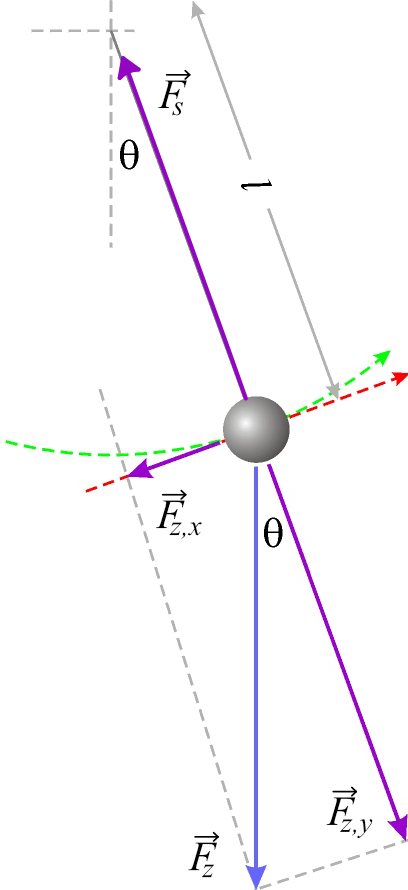
\includegraphics[width=0.34\textwidth]{pendulum}
%\caption{A gull}
\end{wrapfigure}
Volgens de normale richting zal de spankracht in het touw in combinatie met de normale component van de zwaartekracht voor de nodige middelpuntzoekende kracht zorgen. De massa beweegt immers op een cirkel met vari\"erende snelheid waardoor ook een vari\"erende middelpuntzoekende kracht nodig is. Echter kunnen we volgens deze richting niet veel leren over de manier waarop de massa heen en weer slingert. Daarvoor hoeven we enkel de tangenti\"ele richting te bekijken. We passen dan ook de tweede wet van Newton volgens deze richting toe. 
\begin{gather*}
F=ma\\
\Downarrow\\
-mg\sin\theta=m\frac{d^2s}{dt^2}\\
\phantom{\theta=\frac{s}{l}}\Updownarrow\theta=\frac{s}{l}\\
\frac{d^2s}{dt^2}+g\sin\left(\frac{s}{l}\right)=0
\end{gather*}
Dit is een \emph{niet}-lineaire differentiaalvergelijking. Ze is verre van eenvoudig om exact op te lossen. We hebben daartoe een veel zwaarder arsenaal aan wiskundige functies nodig dan dat wij op dit moment kennen. In feite is dat ook niet zo verwonderlijk. Wanneer we bijvoorbeeld de slinger vanuit een initi\"ele hoek van 120 graden met een voldoende hoge beginsnelheid laten vertrekken, zal de slinger niet slingeren maar pulserende rondjes blijven draaien. Deze oplossing samen met bijvoorbeeld stil blijven hangen op 180 graden en nog andere varianten, zijn allemaal mogelijkheden die aan de differentiaalvergelijking moeten voldoen. Ingewikkeld dus.

Wij zullen ons hier beperken tot kleine hoeken\footnote{Ik weet het, dat doet pijn aan het wiskundig exacte deel van ons hart, maar in feite is het in de fysica nooit anders \ldots \'Alles wat we in de fysica doen is een benadering van de realiteit. Zo hebben we bij onze slinger reeds de massa van het touw overboord gegooid, de massa van het object geen dimensie gegeven, gedaan alsof de wrijvingskracht niet bestaat, de zwaartekracht benaderd door $mg$ terwijl die eigenlijk afhankelijk is van de hoogte boven het aardoppervlak, de wetten van Newton gebruikt waar we eigenlijk de wetten van de kwantummechanica zouden moeten bovenhalen, gedaan alsof slingers het enige in het universum zijn \ldots }. In dat geval kunnen we de sinus van een argument benaderen door het argument zelf, $\sin\alpha\approx\alpha$. \footnote{Herinner je misschien dat je ooit de limiet $\displaystyle\lim_{x\rightarrow0}\frac{\sin x}{x}=1$ bewezen hebt.} \footnote{In feite is de wet van Hooke enzelfde lineaire benadering van de veerkracht. Die is ook maar geldig voor zolang we de veer niet te ver uitrekken. Willen we accurater zijn, dan moeten we termen afhankelijk van bijvoorbeeld $x^2$ in rekening brengen \ldots}
\begin{figure}[h]
\centering
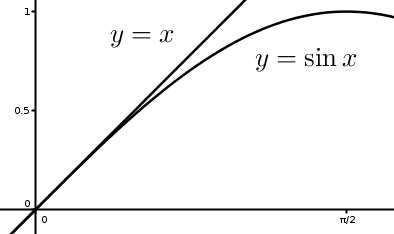
\includegraphics[width=0.4\textwidth]{sinx_x}
\end{figure}
% \begin{minipage}[t]{.5\textwidth}
% \begin{eqnarray*}
% \sin\alpha\approx\alpha
% \end{eqnarray*}
% \end{minipage}
% \begin{minipage}[t]{.4\textwidth}
% \phantom{}
% 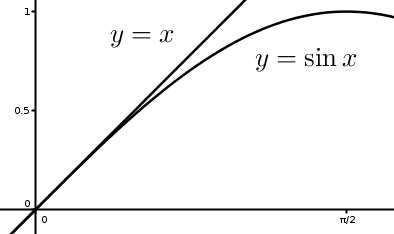
\includegraphics[width=\textwidth]{sinx_x}
% \end{minipage}
\newline
De differentiaalvergelijking wordt er dan een heel pak gemakkelijker op:
\begin{eqnarray*}
\frac{d^2s}{dt^2}+g\sin\left(\frac{s}{l}\right)&=&0\\
&\rotatebox[origin=c]{-90}{$\rightsquigarrow$}&\mathrm{benadering} \sin\alpha\approx\alpha\\
\frac{d^2s}{dt^2}+\frac{g}{l}s&=&0
\end{eqnarray*}
We vinden zo niets anders dan de differentiaalvergelijking van de harmonische trilling (\ref{diffvgl_ht}). De oplossing is wiskundig gezien dan ook dezelfde\footnote{Zo zie je maar hoe we een eenheid in verschillende verschijnselen kunnen terugvinden.}.
\begin{gather*}
\frac{d^2s}{dt^2}+\frac{g}{l}s=0\quad\Leftrightarrow\\
%\Updownarrow\\
s(t)=A\sin(\omega t+\varphi)\quad\mathrm{met}\quad\omega=\sqrt{\frac{g}{l}}
\end{gather*}
Realiseer je dat de amplitude hier de booglengte bij maximale uitwijking is. Ook zien we dat de slingerlengte de periode van de trilling bepaalt en dat de amplitude noch de massa hierop een invloed heeft \ldots
\begin{eqnarray*}
T=2\pi\sqrt{\frac{l}{g}},\quad f=\frac{1}{2\pi}\sqrt{\frac{g}{l}}
\end{eqnarray*}

\newpage

\section{Resonantie}

% microgolfoven

Het verschijnsel resonantie is je zeker bekend. Naar alle waarschijnlijkheid heb je ooit je kleine zusje geduwd op de schommel. Uiteraard deed je dat niet zomaar willekeurig maar met de juiste regelmaat. Je duwde wanneer ze net voorbij het hoogste punt bij jou was -- niet wanneer ze naar je toe kwam! Op die manier ging zij hoger en hoger en nam het plezier alleen maar toe. En dat totdat ze schrik kreeg omdat jij te ver ging \ldots

We beschouwen een model waarin we een massa-veersysteem niet langer vrij laten trillen maar onderwerpen aan een periodieke aandrijvende kracht waarvan we de frequentie controleren. We hebben dan een gedwongen trilling. In ons model kunnen we natuurlijk allerlei soorten manieren van externe krachten steken maar om een differentiaalvergelijking te bekomen die toch ergens hanteerbaar is, nemen we een oscillerende kracht $F=F_0\cos\omega t$ waarin $F_0$ de maximale kracht is waarmee we trekken of duwen en $\omega$ de pulsatie waarmee we de kracht sinuso\"idaal laten vari\"eren. Ook voegen we ditmaal wrijving toe. We nemen een model waarin de wrijvingskracht recht evenredig is met snelheid $F_w=-cv$. Hierin is $c$ een co\"effici\"ent die de sterkte van de demping bepaalt. Het minteken zorgt ervoor dat de component van de wrijvingskracht steeds tegengesteld is aan de snelheid; de wrijvingskracht werkt de beweging altijd tegen. Zolang de snelheid niet te groot wordt, is dit een realistisch model. We vertrekken weer met de tweede wet van Newton:
\begin{gather}
F=ma\nonumber\\
\Downarrow\nonumber\\
-kx-cv+F_0\cos\omega t=ma\nonumber\\
\Updownarrow\nonumber\\
x''+\gamma x'+\omega_0^2x=\frac{F_0}{m}\cos\omega t\label{diffvgl_resonantie}
\end{gather}
Waarin we $c/m$ hebben vervangen door een nieuw symbool $\gamma=c/m$ en ook $\omega_0$ hebben gebruikt voor $\sqrt{k/m}$. $\omega_0=\sqrt{k/m}$ is de natuurlijke pulsatie; de frequentie (op $2\pi$ na) waarmee de massa zou trillen, moest ze vrij worden gelaten.

De oplossing\footnote{Het oplossen van deze vergelijking is relatief eenvoudig wanneer we complexe e-machten gebruiken.\footnotemark Alleen kennen we die nog niet omdat ze alweer gereserveerd zijn voor een vervolgstudie na het 6de. Er moet nog \'iets overblijven om te bestuderen na je humaniora.}\footnotetext{Eenvoudig - complex: heb je'm?} van deze differentiaalvergelijking die overblijft na een zekere tijd wordt gegeven door
\begin{eqnarray*}
x(t)=A\cos(\omega t-\varphi)&\mathrm{met}&
\begin{array}[t]{rcl}
\displaystyle A&=&\frac{F_0/m}{\sqrt{(\omega_0^2-\omega^2)^2+\gamma^2\omega^2}}\\
\displaystyle\tan\varphi&=&\frac{\gamma\omega}{\omega_0^2-\omega^2}
\end{array}
\end{eqnarray*}
Dat betekent dat de massa, na een korte overgangsperiode of nadat de eerste onregelmatige trillingen zijn uitgedoofd, een harmonische trilling zal uitvoeren met dezelfde frequentie als de externe aandrijving. Het bijzondere is echter terug te vinden in de amplitude. We zien dat al naargelang de opgelegde frequentie, we een andere amplitude krijgen. En jawel, als we een grafiek maken van de amplitude in functie van de aandrijving $\omega$ zien we dat in de buurt van de natuurlijke frequentie $\omega_0$ (om precies te zijn, een waarde die net iets kleiner is) de amplitude een sterke piek vertoont. 
\begin{figure}[h]
\centering
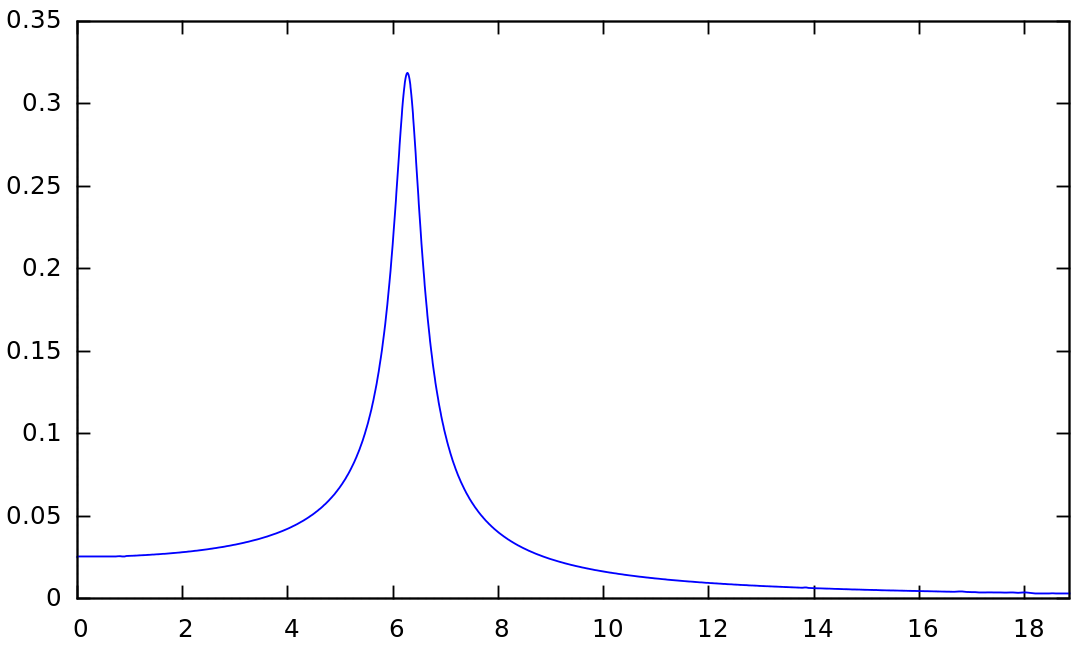
\includegraphics[width=.55\textwidth]{resonantie_curve}
\caption{$A$ in functie van $\omega$.}
\end{figure}
De frequentie waarbij dit optreedt noemen we de \emph{resonantiefrequentie}. Het systeem zal dus bij \'e\'en specifieke frequentie extreem meetrillen. Op de juiste momenten wordt er dus aan de massa geduwd/getrokken zodat er maximaal energie wordt `ingepompt'. Die energie gaat dan natuurlijk weer verloren door de demping.

%Uit de afhankelijkheid van het faseverschil $\varphi$ van de trilling t.o.v. de extern aangelegde trilling, valt op te maken dat bij de resonantiefrequentie het faseverschil $\pi/2$ is; de trilling ijlt een kwart cyclus na op de aandrijving. Naarmate de externe frequentie groter en groter wordt, gaat de massa meer en meer in tegenfase trillen. Het faseverschil nadert $\pi$.
%\begin{figure}[h]
%\centering
%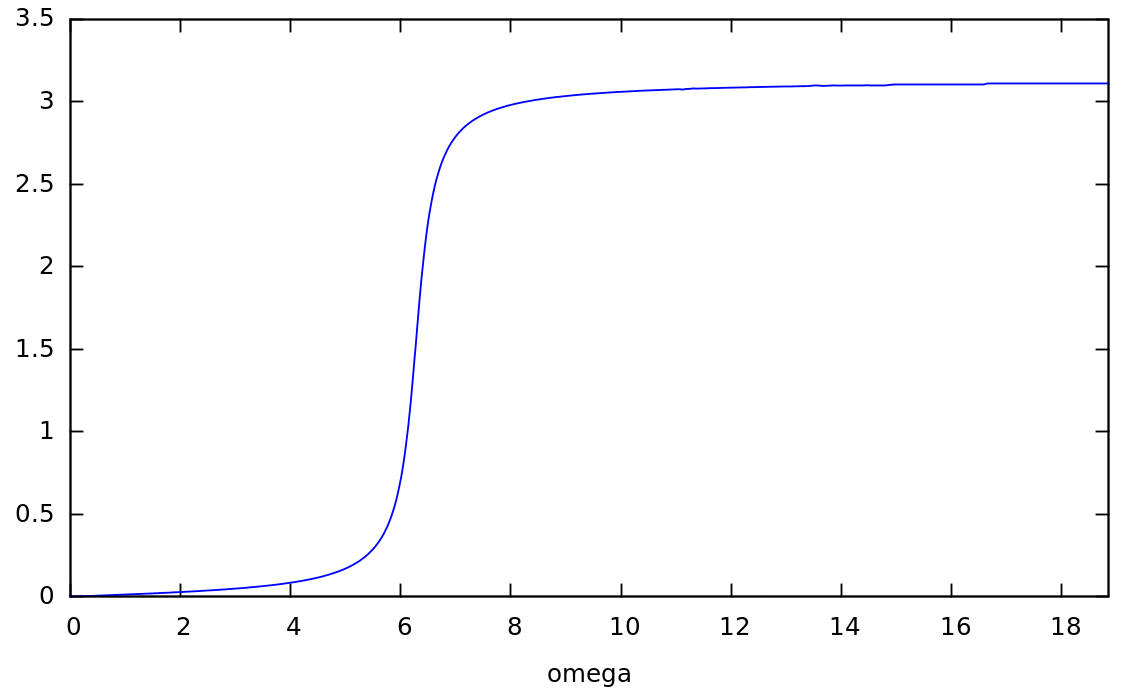
\includegraphics[width=.55\textwidth]{resonantie_fase}
%\caption{$\varphi$ in functie van $\omega$.}
%\end{figure}

%\section{Samenstellen van trillingen}
%- Fourieranalyse?
